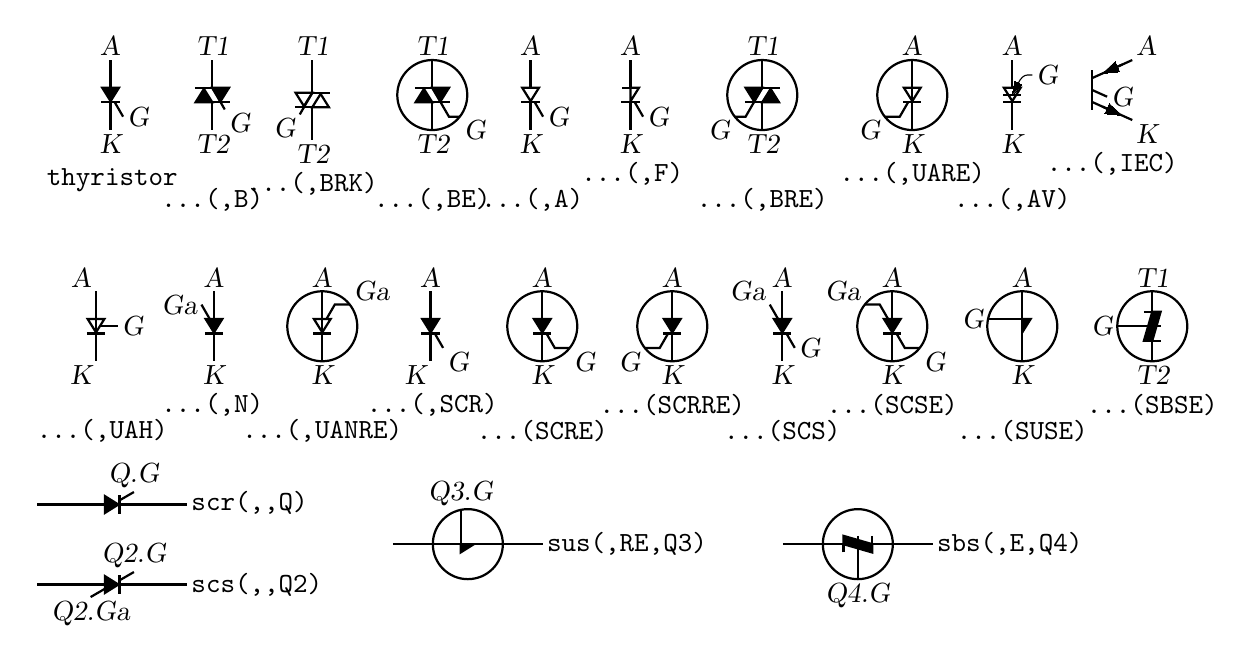
\begin{tikzpicture}[scale=2.54]
% dpic version 2020.03.01 option -g for TikZ and PGF 1.01
\ifx\dpiclw\undefined\newdimen\dpiclw\fi
\global\def\dpicdraw{\draw[line width=\dpiclw]}
\global\def\dpicstop{;}
\dpiclw=0.8bp
\dpiclw=0.8bp
\dpicdraw (-2.38478,-0.179985)
 --(-2.38478,-0.3189)\dpicstop
\global\let\dpicshdraw=\dpicdraw\global\def\dpicdraw{}
\global\def\dpicstop{--}
\dpicshdraw[fill=white!0!black]
\dpicdraw (-2.38478,-0.3189)
 --(-2.343113,-0.3189)
 --(-2.38478,-0.385534)
 --(-2.426446,-0.3189)
 --(-2.38478,-0.3189)\dpicstop
cycle; \global\let\dpicdraw=\dpicshdraw\global\def\dpicstop{;}
\dpicdraw (-2.430498,-0.391069)
 --(-2.339061,-0.391069)\dpicstop
\dpicdraw (-2.363946,-0.391069)
 --(-2.32228,-0.463238)\dpicstop
\dpicdraw (-2.38478,-0.391069)
 --(-2.38478,-0.529985)\dpicstop
\draw (-2.38478,-0.179985) node[above=-2bp]{\sl A};
\draw (-2.38478,-0.529985) node[below=-2bp]{\sl K};
\draw (-2.32228,-0.463238) node[right=-2bp]{\sl G};
\draw (-2.376389,-0.779985) node{\tt thyristor};
\dpicdraw (-1.876389,-0.179985)
 --(-1.876389,-0.3189)\dpicstop
\dpicdraw (-1.876389,-0.3189)
 --(-1.813889,-0.427154)\dpicstop
\global\let\dpicshdraw=\dpicdraw\global\def\dpicdraw{}
\global\def\dpicstop{--}
\dpicshdraw[fill=white!0!black]
\dpicdraw (-1.834722,-0.3189)
 --(-1.793056,-0.3189)
 --(-1.834722,-0.385534)
 --(-1.876389,-0.3189)
 --(-1.834722,-0.3189)\dpicstop
cycle; \global\let\dpicdraw=\dpicshdraw\global\def\dpicstop{;}
\dpicdraw (-1.963774,-0.391069)
 --(-1.789004,-0.391069)\dpicstop
\dpicdraw (-1.963774,-0.3189)
 --(-1.789004,-0.3189)\dpicstop
\global\let\dpicshdraw=\dpicdraw\global\def\dpicdraw{}
\global\def\dpicstop{--}
\dpicshdraw[fill=white!0!black]
\dpicdraw (-1.918056,-0.391069)
 --(-1.876389,-0.391069)
 --(-1.918056,-0.324435)
 --(-1.959722,-0.391069)
 --(-1.918056,-0.391069)\dpicstop
cycle; \global\let\dpicdraw=\dpicshdraw\global\def\dpicstop{;}
\dpicdraw (-1.876389,-0.391069)
 --(-1.876389,-0.529985)\dpicstop
\draw (-1.876389,-0.179985) node[above=-2bp]{\sl T1};
\draw (-1.876389,-0.529985) node[below=-2bp]{\sl T2};
\draw (-1.813889,-0.427154) node[below right=-2bp]{\sl G};
\draw (-1.876389,-0.879985) node{\tt ...(,B)};
\dpicdraw (-1.376389,-0.179985)
 --(-1.376389,-0.3439)\dpicstop
\dpicdraw (-1.376389,-0.3439)
 --(-1.438889,-0.452154)\dpicstop
\dpicdraw (-1.418056,-0.3439)
 --(-1.376389,-0.3439)
 --(-1.418056,-0.410534)
 --(-1.459722,-0.3439)
 --(-1.418056,-0.3439)\dpicstop
\dpicdraw (-1.463774,-0.416069)
 --(-1.289004,-0.416069)\dpicstop
\dpicdraw (-1.463774,-0.3439)
 --(-1.289004,-0.3439)\dpicstop
\dpicdraw (-1.334722,-0.416069)
 --(-1.293056,-0.416069)
 --(-1.334722,-0.349435)
 --(-1.376389,-0.416069)
 --(-1.334722,-0.416069)\dpicstop
\dpicdraw (-1.376389,-0.416069)
 --(-1.376389,-0.579985)\dpicstop
\draw (-1.376389,-0.179985) node[above=-2bp]{\sl T1};
\draw (-1.376389,-0.579985) node[below=-2bp]{\sl T2};
\draw (-1.438889,-0.452154) node[below left=-2bp]{\sl G};
\draw (-1.376389,-0.799985) node{\tt ...(,BRK)};
\dpicdraw (-0.776389,-0.179985)
 --(-0.776389,-0.3189)\dpicstop
\dpicdraw (-0.776389,-0.3189)
 --(-0.693056,-0.463238)
 --(-0.637945,-0.463238)\dpicstop
\global\let\dpicshdraw=\dpicdraw\global\def\dpicdraw{}
\global\def\dpicstop{--}
\dpicshdraw[fill=white!0!black]
\dpicdraw (-0.734722,-0.3189)
 --(-0.693056,-0.3189)
 --(-0.734722,-0.385534)
 --(-0.776389,-0.3189)
 --(-0.734722,-0.3189)\dpicstop
cycle; \global\let\dpicdraw=\dpicshdraw\global\def\dpicstop{;}
\dpicdraw (-0.863774,-0.391069)
 --(-0.689004,-0.391069)\dpicstop
\dpicdraw (-0.863774,-0.3189)
 --(-0.689004,-0.3189)\dpicstop
\global\let\dpicshdraw=\dpicdraw\global\def\dpicdraw{}
\global\def\dpicstop{--}
\dpicshdraw[fill=white!0!black]
\dpicdraw (-0.818056,-0.391069)
 --(-0.776389,-0.391069)
 --(-0.818056,-0.324435)
 --(-0.859722,-0.391069)
 --(-0.818056,-0.391069)\dpicstop
cycle; \global\let\dpicdraw=\dpicshdraw\global\def\dpicstop{;}
\dpicdraw (-0.776389,-0.391069)
 --(-0.776389,-0.529985)\dpicstop
\dpicdraw (-0.776389,-0.354985) circle (0.068898in)\dpicstop
\draw (-0.776389,-0.179985) node[above=-2bp]{\sl T1};
\draw (-0.776389,-0.529985) node[below=-2bp]{\sl T2};
\draw (-0.637945,-0.463238) node[below right=-2bp]{\sl G};
\draw (-0.776389,-0.879985) node{\tt ...(,BE)};
\dpicdraw (-0.28478,-0.179985)
 --(-0.28478,-0.3189)\dpicstop
\dpicdraw (-0.28478,-0.3189)
 --(-0.243113,-0.3189)
 --(-0.28478,-0.385534)
 --(-0.326446,-0.3189)
 --(-0.28478,-0.3189)\dpicstop
\dpicdraw (-0.330498,-0.391069)
 --(-0.239061,-0.391069)\dpicstop
\dpicdraw (-0.263946,-0.391069)
 --(-0.22228,-0.463238)\dpicstop
\dpicdraw (-0.28478,-0.391069)
 --(-0.28478,-0.529985)\dpicstop
\draw (-0.28478,-0.179985) node[above=-2bp]{\sl A};
\draw (-0.28478,-0.529985) node[below=-2bp]{\sl K};
\draw (-0.22228,-0.463238) node[right=-2bp]{\sl G};
\draw (-0.276389,-0.879985) node{\tt ...(,A)};
\dpicdraw (0.21522,-0.179985)
 --(0.21522,-0.3189)\dpicstop
\dpicdraw (0.21522,-0.3189)
 --(0.256887,-0.3189)
 --(0.21522,-0.385534)
 --(0.21522,-0.3189)\dpicstop
\dpicdraw (0.21522,-0.3189)
 --(0.173554,-0.3189)\dpicstop
\dpicdraw (0.169502,-0.391069)
 --(0.260939,-0.391069)\dpicstop
\dpicdraw (0.236054,-0.391069)
 --(0.27772,-0.463238)\dpicstop
\dpicdraw (0.21522,-0.391069)
 --(0.21522,-0.529985)\dpicstop
\draw (0.21522,-0.179985) node[above=-2bp]{\sl A};
\draw (0.21522,-0.529985) node[below=-2bp]{\sl K};
\draw (0.27772,-0.463238) node[right=-2bp]{\sl G};
\draw (0.223611,-0.749985) node{\tt ...(,F)};
\dpicdraw (0.873611,-0.179985)
 --(0.873611,-0.3189)\dpicstop
\dpicdraw (0.873611,-0.3189)
 --(0.790278,-0.463238)
 --(0.735167,-0.463238)\dpicstop
\global\let\dpicshdraw=\dpicdraw\global\def\dpicdraw{}
\global\def\dpicstop{--}
\dpicshdraw[fill=white!0!black]
\dpicdraw (0.831944,-0.3189)
 --(0.873611,-0.3189)
 --(0.831944,-0.385534)
 --(0.790278,-0.3189)
 --(0.831944,-0.3189)\dpicstop
cycle; \global\let\dpicdraw=\dpicshdraw\global\def\dpicstop{;}
\dpicdraw (0.786226,-0.391069)
 --(0.960996,-0.391069)\dpicstop
\dpicdraw (0.786226,-0.3189)
 --(0.960996,-0.3189)\dpicstop
\global\let\dpicshdraw=\dpicdraw\global\def\dpicdraw{}
\global\def\dpicstop{--}
\dpicshdraw[fill=white!0!black]
\dpicdraw (0.915278,-0.391069)
 --(0.956944,-0.391069)
 --(0.915278,-0.324435)
 --(0.873611,-0.391069)
 --(0.915278,-0.391069)\dpicstop
cycle; \global\let\dpicdraw=\dpicshdraw\global\def\dpicstop{;}
\dpicdraw (0.873611,-0.391069)
 --(0.873611,-0.529985)\dpicstop
\dpicdraw (0.873611,-0.354985) circle (0.068898in)\dpicstop
\draw (0.873611,-0.179985) node[above=-2bp]{\sl T1};
\draw (0.873611,-0.529985) node[below=-2bp]{\sl T2};
\draw (0.735167,-0.463238) node[below left=-2bp]{\sl G};
\draw (0.873611,-0.879985) node{\tt ...(,BRE)};
\dpicdraw (1.623611,-0.179985)
 --(1.623611,-0.3189)\dpicstop
\dpicdraw (1.623611,-0.3189)
 --(1.665278,-0.3189)
 --(1.623611,-0.385534)
 --(1.581944,-0.3189)
 --(1.623611,-0.3189)\dpicstop
\dpicdraw (1.623611,-0.3189)
 --(1.623611,-0.391069)\dpicstop
\dpicdraw (1.577893,-0.391069)
 --(1.66933,-0.391069)\dpicstop
\dpicdraw (1.602778,-0.391069)
 --(1.561111,-0.463238)
 --(1.486111,-0.463238)\dpicstop
\dpicdraw (1.623611,-0.391069)
 --(1.623611,-0.529985)\dpicstop
\dpicdraw (1.623611,-0.354985) circle (0.068898in)\dpicstop
\draw (1.623611,-0.179985) node[above=-2bp]{\sl A};
\draw (1.623611,-0.529985) node[below=-2bp]{\sl K};
\draw (1.486111,-0.463238) node[below left=-2bp]{\sl G};
\draw (1.623611,-0.749985) node{\tt ...(,UARE)};
\dpicdraw (2.123611,-0.179985)
 --(2.123611,-0.3189)\dpicstop
\dpicdraw (2.123611,-0.3189)
 --(2.165278,-0.3189)
 --(2.123611,-0.385534)
 --(2.081944,-0.3189)
 --(2.123611,-0.3189)\dpicstop
\dpicdraw (2.077893,-0.354985)
 --(2.16933,-0.354985)\dpicstop
\dpicdraw (2.077893,-0.391069)
 --(2.16933,-0.391069)\dpicstop
\dpicdraw (2.123611,-0.391069)
 --(2.123611,-0.529985)\dpicstop
\dpiclw=0.4bp
\filldraw[line width=0bp](2.135537,-0.286412)
 --(2.123611,-0.354985)
 --(2.171314,-0.304301) --cycle\dpicstop
\dpicdraw (2.223611,-0.254985)
 --(2.198611,-0.254985)
 ..controls (2.181944,-0.254985) and (2.166719,-0.268769)
 ..(2.152934,-0.296338)
 --(2.132257,-0.337692)\dpicstop
\dpiclw=0.8bp
\draw (2.123611,-0.179985) node[above=-2bp]{\sl A};
\draw (2.123611,-0.529985) node[below=-2bp]{\sl K};
\draw (2.223611,-0.254985) node[right=-2bp]{\sl G};
\draw (2.123611,-0.879985) node{\tt ...(,AV)};
\dpicdraw (2.523611,-0.229985)
 --(2.523611,-0.429985)\dpicstop
\dpicdraw (2.723611,-0.179985)
 --(2.523611,-0.269985)\dpicstop
\filldraw[line width=0bp](2.638206,-0.187957)
 --(2.573611,-0.247485)
 --(2.661004,-0.238619) --cycle\dpicstop
\dpicdraw (2.673611,-0.202485)
 --(2.589632,-0.240275)\dpicstop
\dpicdraw (2.723611,-0.479985)
 --(2.523611,-0.389985)\dpicstop
\filldraw[line width=0bp](2.586219,-0.448619)
 --(2.673611,-0.457485)
 --(2.609017,-0.397957) --cycle\dpicstop
\dpicdraw (2.65759,-0.450275)
 --(2.573611,-0.412485)\dpicstop
\dpicdraw (2.523611,-0.329985)
 --(2.597685,-0.363318)\dpicstop
\draw (2.723611,-0.179985) node[above right=-2bp]{\sl A};
\draw (2.723611,-0.479985) node[below right=-2bp]{\sl K};
\draw (2.597685,-0.363318) node[right=-2bp]{\sl G};
\draw (2.623611,-0.699985) node{\tt ...(,IEC)};
\dpicdraw (-2.457639,-1.336073)
 --(-2.457639,-1.474989)\dpicstop
\dpicdraw (-2.457639,-1.474989)
 --(-2.415972,-1.474989)
 --(-2.457639,-1.541623)
 --(-2.499306,-1.474989)
 --(-2.457639,-1.474989)\dpicstop
\dpicdraw (-2.457639,-1.474989)
 --(-2.457639,-1.547157)\dpicstop
\dpicdraw (-2.436806,-1.511073)
 --(-2.34942,-1.511073)\dpicstop
\dpicdraw (-2.503357,-1.547157)
 --(-2.41192,-1.547157)\dpicstop
\dpicdraw (-2.457639,-1.547157)
 --(-2.457639,-1.686073)\dpicstop
\draw (-2.457639,-1.336073) node[above left=-2bp]{\sl A};
\draw (-2.457639,-1.686073) node[below left=-2bp]{\sl K};
\draw (-2.34942,-1.511073) node[right=-2bp]{\sl G};
\draw (-2.426389,-2.036073) node{\tt ...(,UAH)};
\dpicdraw (-1.867998,-1.336073)
 --(-1.867998,-1.474989)\dpicstop
\global\let\dpicshdraw=\dpicdraw\global\def\dpicdraw{}
\global\def\dpicstop{--}
\dpicshdraw[fill=white!0!black]
\dpicdraw (-1.867998,-1.474989)
 --(-1.826331,-1.474989)
 --(-1.867998,-1.541623)
 --(-1.909665,-1.474989)
 --(-1.867998,-1.474989)\dpicstop
cycle; \global\let\dpicdraw=\dpicshdraw\global\def\dpicstop{;}
\dpicdraw (-1.913717,-1.547157)
 --(-1.82228,-1.547157)\dpicstop
\dpicdraw (-1.888831,-1.474989)
 --(-1.930498,-1.40282)\dpicstop
\dpicdraw (-1.867998,-1.547157)
 --(-1.867998,-1.686073)\dpicstop
\draw (-1.867998,-1.336073) node[above=-2bp]{\sl A};
\draw (-1.867998,-1.686073) node[below=-2bp]{\sl K};
\draw (-1.930498,-1.40282) node[left=-2bp]{\sl Ga};
\draw (-1.876389,-1.906073) node{\tt ...(,N)};
\dpicdraw (-1.326389,-1.336073)
 --(-1.326389,-1.474989)\dpicstop
\dpicdraw (-1.326389,-1.474989)
 --(-1.284722,-1.474989)
 --(-1.326389,-1.541623)
 --(-1.368056,-1.474989)
 --(-1.326389,-1.474989)\dpicstop
\dpicdraw (-1.326389,-1.474989)
 --(-1.326389,-1.547157)\dpicstop
\dpicdraw (-1.372107,-1.547157)
 --(-1.28067,-1.547157)\dpicstop
\dpicdraw (-1.305556,-1.474989)
 --(-1.263889,-1.40282)
 --(-1.188889,-1.40282)\dpicstop
\dpicdraw (-1.326389,-1.547157)
 --(-1.326389,-1.686073)\dpicstop
\dpicdraw (-1.326389,-1.511073) circle (0.068898in)\dpicstop
\draw (-1.326389,-1.336073) node[above=-2bp]{\sl A};
\draw (-1.326389,-1.686073) node[below=-2bp]{\sl K};
\draw (-1.188889,-1.40282) node[above right=-2bp]{\sl Ga};
\draw (-1.326389,-2.036073) node{\tt ...(,UANRE)};
\dpicdraw (-0.78478,-1.336073)
 --(-0.78478,-1.474989)\dpicstop
\global\let\dpicshdraw=\dpicdraw\global\def\dpicdraw{}
\global\def\dpicstop{--}
\dpicshdraw[fill=white!0!black]
\dpicdraw (-0.78478,-1.474989)
 --(-0.743113,-1.474989)
 --(-0.78478,-1.541623)
 --(-0.826446,-1.474989)
 --(-0.78478,-1.474989)\dpicstop
cycle; \global\let\dpicdraw=\dpicshdraw\global\def\dpicstop{;}
\dpicdraw (-0.830498,-1.547157)
 --(-0.739061,-1.547157)\dpicstop
\dpicdraw (-0.763946,-1.547157)
 --(-0.72228,-1.619326)\dpicstop
\dpicdraw (-0.78478,-1.547157)
 --(-0.78478,-1.686073)\dpicstop
\draw (-0.78478,-1.336073) node[above=-2bp]{\sl A};
\draw (-0.78478,-1.686073) node[below left=-2bp]{\sl K};
\draw (-0.72228,-1.619326) node[below right=-2bp]{\sl G};
\draw (-0.776389,-1.906073) node{\tt ...(,SCR)};
\dpicdraw (-0.226389,-1.336073)
 --(-0.226389,-1.474989)\dpicstop
\global\let\dpicshdraw=\dpicdraw\global\def\dpicdraw{}
\global\def\dpicstop{--}
\dpicshdraw[fill=white!0!black]
\dpicdraw (-0.226389,-1.474989)
 --(-0.184722,-1.474989)
 --(-0.226389,-1.541623)
 --(-0.268056,-1.474989)
 --(-0.226389,-1.474989)\dpicstop
cycle; \global\let\dpicdraw=\dpicshdraw\global\def\dpicstop{;}
\dpicdraw (-0.272107,-1.547157)
 --(-0.18067,-1.547157)\dpicstop
\dpicdraw (-0.205556,-1.547157)
 --(-0.163889,-1.619326)
 --(-0.088889,-1.619326)\dpicstop
\dpicdraw (-0.226389,-1.547157)
 --(-0.226389,-1.686073)\dpicstop
\dpicdraw (-0.226389,-1.511073) circle (0.068898in)\dpicstop
\draw (-0.226389,-1.336073) node[above=-2bp]{\sl A};
\draw (-0.226389,-1.686073) node[below=-2bp]{\sl K};
\draw (-0.088889,-1.619326) node[below right=-2bp]{\sl G};
\draw (-0.226389,-2.036073) node{\tt ...(SCRE)};
\dpicdraw (0.423611,-1.336073)
 --(0.423611,-1.474989)\dpicstop
\global\let\dpicshdraw=\dpicdraw\global\def\dpicdraw{}
\global\def\dpicstop{--}
\dpicshdraw[fill=white!0!black]
\dpicdraw (0.423611,-1.474989)
 --(0.465278,-1.474989)
 --(0.423611,-1.541623)
 --(0.381944,-1.474989)
 --(0.423611,-1.474989)\dpicstop
cycle; \global\let\dpicdraw=\dpicshdraw\global\def\dpicstop{;}
\dpicdraw (0.377893,-1.547157)
 --(0.46933,-1.547157)\dpicstop
\dpicdraw (0.402778,-1.547157)
 --(0.361111,-1.619326)
 --(0.286111,-1.619326)\dpicstop
\dpicdraw (0.423611,-1.547157)
 --(0.423611,-1.686073)\dpicstop
\dpicdraw (0.423611,-1.511073) circle (0.068898in)\dpicstop
\draw (0.423611,-1.336073) node[above=-2bp]{\sl A};
\draw (0.423611,-1.686073) node[below=-2bp]{\sl K};
\draw (0.286111,-1.619326) node[below left=-2bp]{\sl G};
\draw (0.423611,-1.906073) node{\tt ...(SCRRE)};
\dpicdraw (0.973611,-1.336073)
 --(0.973611,-1.474989)\dpicstop
\global\let\dpicshdraw=\dpicdraw\global\def\dpicdraw{}
\global\def\dpicstop{--}
\dpicshdraw[fill=white!0!black]
\dpicdraw (0.973611,-1.474989)
 --(1.015278,-1.474989)
 --(0.973611,-1.541623)
 --(0.931944,-1.474989)
 --(0.973611,-1.474989)\dpicstop
cycle; \global\let\dpicdraw=\dpicshdraw\global\def\dpicstop{;}
\dpicdraw (0.927893,-1.547157)
 --(1.01933,-1.547157)\dpicstop
\dpicdraw (0.952778,-1.474989)
 --(0.911111,-1.40282)\dpicstop
\dpicdraw (0.994444,-1.547157)
 --(1.036111,-1.619326)\dpicstop
\dpicdraw (0.973611,-1.547157)
 --(0.973611,-1.686073)\dpicstop
\draw (0.973611,-1.336073) node[above=-2bp]{\sl A};
\draw (0.973611,-1.686073) node[below=-2bp]{\sl K};
\draw (1.036111,-1.619326) node[right=-2bp]{\sl G};
\draw (0.973611,-2.036073) node{\tt ...(SCS)};
\draw (0.911111,-1.40282) node[above left=-2bp]{\sl Ga};
\dpicdraw (1.523611,-1.336073)
 --(1.523611,-1.474989)\dpicstop
\global\let\dpicshdraw=\dpicdraw\global\def\dpicdraw{}
\global\def\dpicstop{--}
\dpicshdraw[fill=white!0!black]
\dpicdraw (1.523611,-1.474989)
 --(1.565278,-1.474989)
 --(1.523611,-1.541623)
 --(1.481944,-1.474989)
 --(1.523611,-1.474989)\dpicstop
cycle; \global\let\dpicdraw=\dpicshdraw\global\def\dpicstop{;}
\dpicdraw (1.477893,-1.547157)
 --(1.56933,-1.547157)\dpicstop
\dpicdraw (1.502778,-1.474989)
 --(1.461111,-1.40282)
 --(1.386111,-1.40282)\dpicstop
\dpicdraw (1.544444,-1.547157)
 --(1.586111,-1.619326)
 --(1.661111,-1.619326)\dpicstop
\dpicdraw (1.523611,-1.547157)
 --(1.523611,-1.686073)\dpicstop
\dpicdraw (1.523611,-1.511073) circle (0.068898in)\dpicstop
\draw (1.523611,-1.336073) node[above=-2bp]{\sl A};
\draw (1.523611,-1.686073) node[below=-2bp]{\sl K};
\draw (1.661111,-1.619326) node[below right=-2bp]{\sl G};
\draw (1.523611,-1.906073) node{\tt ...(SCSE)};
\draw (1.386111,-1.40282) node[above left=-2bp]{\sl Ga};
\dpicdraw (2.173611,-1.336073)
 --(2.173611,-1.474989)\dpicstop
\global\let\dpicshdraw=\dpicdraw\global\def\dpicdraw{}
\global\def\dpicstop{--}
\dpicshdraw[fill=white!0!black]
\dpicdraw (2.173611,-1.474989)
 --(2.215278,-1.474989)
 --(2.173611,-1.541623)
 --(2.173611,-1.474989)\dpicstop
cycle; \global\let\dpicdraw=\dpicshdraw\global\def\dpicstop{;}
\dpicdraw (2.173611,-1.474989)
 --(2.002372,-1.474989)\dpicstop
\dpicdraw (2.173611,-1.547157)
 --(2.173611,-1.686073)\dpicstop
\dpicdraw (2.173611,-1.511073) circle (0.068898in)\dpicstop
\draw (2.173611,-1.336073) node[above=-2bp]{\sl A};
\draw (2.173611,-1.686073) node[below=-2bp]{\sl K};
\draw (2.002372,-1.474989) node[left=-2bp]{\sl G};
\draw (2.173611,-2.036073) node{\tt ...(SUSE)};
\dpicdraw (2.823611,-1.336073)
 --(2.823611,-1.438904)\dpicstop
\dpicdraw (2.781944,-1.438904)
 --(2.823611,-1.438904)\dpicstop
\global\let\dpicshdraw=\dpicdraw\global\def\dpicdraw{}
\global\def\dpicstop{--}
\dpicshdraw[fill=white!0!black]
\dpicdraw (2.823611,-1.438904)
 --(2.865278,-1.438904)
 --(2.823611,-1.583242)
 --(2.781944,-1.583242)
 --(2.823611,-1.438904)\dpicstop
cycle; \global\let\dpicdraw=\dpicshdraw\global\def\dpicstop{;}
\dpicdraw (2.865278,-1.583242)
 --(2.823611,-1.583242)\dpicstop
\dpicdraw (2.865278,-1.511073)
 --(2.648611,-1.511073)\dpicstop
\dpicdraw (2.823611,-1.583242)
 --(2.823611,-1.686073)\dpicstop
\dpicdraw (2.823611,-1.511073) circle (0.068898in)\dpicstop
\draw (2.823611,-1.336073) node[above=-2bp]{\sl T1};
\draw (2.823611,-1.686073) node[below=-2bp]{\sl T2};
\draw (2.648611,-1.511073) node[left=-2bp]{\sl G};
\draw (2.823611,-1.906073) node{\tt ...(SBSE)};
\dpicdraw (-2.751389,-2.402454)
 --(-2.412473,-2.402454)\dpicstop
\global\let\dpicshdraw=\dpicdraw\global\def\dpicdraw{}
\global\def\dpicstop{--}
\dpicshdraw[fill=white!0!black]
\dpicdraw (-2.412473,-2.402454)
 --(-2.412473,-2.360788)
 --(-2.345839,-2.402454)
 --(-2.412473,-2.444121)
 --(-2.412473,-2.402454)\dpicstop
cycle; \global\let\dpicdraw=\dpicshdraw\global\def\dpicstop{;}
\dpicdraw (-2.340304,-2.448173)
 --(-2.340304,-2.356736)\dpicstop
\dpicdraw (-2.340304,-2.381621)
 --(-2.268136,-2.339954)\dpicstop
\dpicdraw (-2.340304,-2.402454)
 --(-2.001389,-2.402454)\dpicstop
\draw (-2.001389,-2.394064) node[right=-2bp]{\tt scr(,{,}Q)};
\draw (-2.268136,-2.339954) node[above=-2bp]{\sl Q.G};
\dpicdraw (-2.751389,-2.802454)
 --(-2.412473,-2.802454)\dpicstop
\global\let\dpicshdraw=\dpicdraw\global\def\dpicdraw{}
\global\def\dpicstop{--}
\dpicshdraw[fill=white!0!black]
\dpicdraw (-2.412473,-2.802454)
 --(-2.412473,-2.760788)
 --(-2.345839,-2.802454)
 --(-2.412473,-2.844121)
 --(-2.412473,-2.802454)\dpicstop
cycle; \global\let\dpicdraw=\dpicshdraw\global\def\dpicstop{;}
\dpicdraw (-2.340304,-2.848173)
 --(-2.340304,-2.756736)\dpicstop
\dpicdraw (-2.412473,-2.823288)
 --(-2.484642,-2.864954)\dpicstop
\dpicdraw (-2.340304,-2.781621)
 --(-2.268136,-2.739954)\dpicstop
\dpicdraw (-2.340304,-2.802454)
 --(-2.001389,-2.802454)\dpicstop
\draw (-2.001389,-2.802454) node[right=-2bp]{\tt scs(,{,}Q2)};
\draw (-2.268136,-2.739954) node[above=-2bp]{\sl Q2.G};
\draw (-2.484642,-2.864954) node[below=-2bp]{\sl Q2.Ga};
\dpicdraw (-0.973611,-2.600574)
 --(-0.634696,-2.600574)\dpicstop
\global\let\dpicshdraw=\dpicdraw\global\def\dpicdraw{}
\global\def\dpicstop{--}
\dpicshdraw[fill=white!0!black]
\dpicdraw (-0.634696,-2.600574)
 --(-0.634696,-2.642241)
 --(-0.568062,-2.600574)
 --(-0.634696,-2.600574)\dpicstop
cycle; \global\let\dpicdraw=\dpicshdraw\global\def\dpicstop{;}
\dpicdraw (-0.634696,-2.600574)
 --(-0.634696,-2.429335)\dpicstop
\dpicdraw (-0.562527,-2.600574)
 --(-0.223611,-2.600574)\dpicstop
\dpicdraw (-0.598611,-2.600574) circle (0.068898in)\dpicstop
\draw (-0.223611,-2.600574) node[right=-2bp]{\tt sus(,RE,Q3)};
\draw (-0.634696,-2.429335) node[above=-2bp]{\sl Q3.G};
\dpicdraw (0.976389,-2.600574)
 --(1.27922,-2.600574)\dpicstop
\dpicdraw (1.27922,-2.642241)
 --(1.27922,-2.600574)\dpicstop
\global\let\dpicshdraw=\dpicdraw\global\def\dpicdraw{}
\global\def\dpicstop{--}
\dpicshdraw[fill=white!0!black]
\dpicdraw (1.27922,-2.600574)
 --(1.27922,-2.558907)
 --(1.423558,-2.600574)
 --(1.423558,-2.642241)
 --(1.27922,-2.600574)\dpicstop
cycle; \global\let\dpicdraw=\dpicshdraw\global\def\dpicstop{;}
\dpicdraw (1.423558,-2.558907)
 --(1.423558,-2.600574)\dpicstop
\dpicdraw (1.351389,-2.558907)
 --(1.351389,-2.775574)\dpicstop
\dpicdraw (1.423558,-2.600574)
 --(1.726389,-2.600574)\dpicstop
\dpicdraw (1.351389,-2.600574) circle (0.068898in)\dpicstop
\draw (1.726389,-2.600574) node[right=-2bp]{\tt sbs(,E,Q4)};
\draw (1.351389,-2.775574) node[below=-2bp]{\sl Q4.G};
\end{tikzpicture}
\vspace*{-0.5\baselineskip}
